\documentclass[ngerman]{beamer}
\usepackage{etex}
\usepackage[beamer]{mydefs}
\usepackage{calc}
\usepackage{babel}
\usepackage{fontspec}
\usepackage{textpos}

%%%

\title{Lernen Terminologischen Wissens\\ mit hoher Konfidenz aus fehlerhaften Daten}
\author{Daniel Borchmann}
\date{9.\,September 2014}

%%%

\includeonlyframes{current}
\usetikzlibrary{decorations.pathmorphing,calc,arrows}
\tikzset{>={stealth'[sep]}}

% \let\oldemph\emph
% \renewcommand{\emph}[1]{\alert<.>{\oldemph{#1}}}

%%%

\begin{document}

\begin{frame}[plain]
  \maketitle
\end{frame}

\begin{frame}

  \onslide<1->

  \begin{block}{Ziel}
    Wissen aus Daten für maschinelle Bearbeitung extrahieren
  \end{block}

  \onslide<2->

  \begin{block}{Beobachtung}
    \begin{itemize}
    \item<3-> faktisches Wissen leicht extrahierbar
    \item<8-> terminologisches (begriffliches) Wissen schwer extrahierbar
    \end{itemize}
  \end{block}

  \onslide<4->

  \vspace*{-0.6\baselineskip}
  \begin{overlayarea}{\linewidth}{13ex}
    \only<4-6>{
      \begin{Beispiel}[DBpedia/Wikidata]
        \only<5->{
          \begin{center}\ttfamily
            <http://dbpedia.org/resource/\alert<6->{Aldous\_Huxley}>\\
            <http://dbpedia.org/ontology/\alert<6->{notableWork}>\\
            <http://dbpedia.org/resource/\alert<6->{Brave\_New\_World}> .
          \end{center}
        }
      \end{Beispiel}
    }
    
    \only<9->{
      \begin{Beispiel}
        \begin{itemize}
        \item<10-> Jede Katze ist ein Säugetier
        \item<11-> Hunde sind keine Katzen
        \item<12-> Jeder Mensch, der ein Kind hat, ist ein Elternteil
        \end{itemize}
      \end{Beispiel}
    }
  \end{overlayarea}

\end{frame}

\begin{frame}

  \onslide<1->

  \begin{block}{Grundlegende Fragen}
    \begin{itemize}
    \item<2-> Wie Wissen darstellen? \visible<5->{$\quad\Rightarrow\quad$
        \emph{Beschreibungslogiken} }
    \item<3-> Wie Wissen extrahieren? \visible<10->{$\quad\Rightarrow\quad$ \emph{Formale
          Begriffsanalyse}}
    \item<4-> Welches Wissen extrahieren? \visible<11->{$\quad\Rightarrow\quad$
        \emph{\enquote{interessantes}}}
    \end{itemize}
  \end{block}

  \onslide<6->

  \begin{Beispiel}[General Concept Inclusions, GCIs]
    \begin{itemize}
    \item<7-> $\mathsf{Cat} \sqsubseteq \mathsf{Mammal}$
    \item<8-> $\mathsf{Dog} \sqcap \mathsf{Cat} \sqsubseteq \bot$
    \item<9-> $\exists \mathsf{child}. \top \sqsubseteq \mathsf{Parent}$
    \end{itemize}
  \end{Beispiel}

\end{frame}

\begin{frame}

  \onslide<+->
  
  \centering
  
  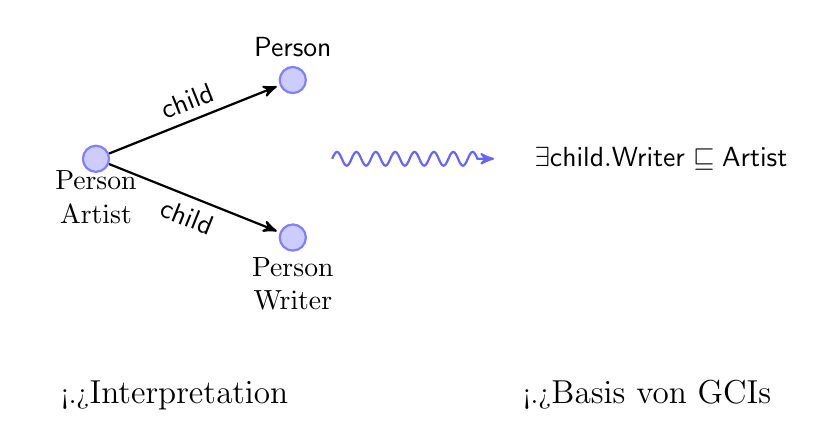
\begin{tikzpicture}[element/.style = {circle,draw=blue!50,fill=blue!20,thick}]
    \node[element, draw, circle, label=below:{\parbox{1.5cm}{\vspace*{-.5cm}\center
        Person\\Artist}}] (B) at (3,-1) {};
    \node[element, draw, circle, label=above:{\sf Person}] (C) at (5.5,0) {};
    \node[element, draw, circle, label=below:{\parbox{1.5cm}{\vspace*{-.4cm}\center
        Person\\Writer}}] (D) at (5.5,-2) {};
    \path[->,thick]
    (B) edge node[midway,above,sloped] {\sf child} (C)
    (B) edge node[midway,below,sloped] {\sf child} (D)
    ;

    \node[coordinate] (D) at (6,-1) {};

    \onslide<+->{
      \node  (E) at (10,-1) {$\quad\mathsf{\exists child.Writer} \sqsubseteq \mathsf{Artist}$};
      \draw[->,thick,blue!60,opaque=50,decorate,decoration={coil,aspect=0,post length=0.7em,
        segment length=0.7em}] (D) to (E);
    }

    \onslide<+->{
      \node at (4, -4) {\alert<.>{\large Interpretation}};
    }

    \onslide<+->{
      \node at (10, -4) {\alert<.>{\large Basis von GCIs}};
    }
  \end{tikzpicture}
  
\end{frame}

\begin{frame}

  \onslide<+->

  Fixiere disjunkte Mengen $N_{C}$ (Konzeptnamen) und $N_{R}$ (Rollennamen).

  \onslide<+->

  \begin{Definition}
    \emph{$\ELbot$-Konzeptbeschreibungen} $C$ sind von der Form
    \begin{equation*}
      C ::= A \mid C \sqcap\! C \mid \exists r. C \mid \bot \mid \top
    \end{equation*}
    für $A \in N_C, r \in N_R$.
  \end{Definition}

  \onslide<+->

  \begin{Beispiel}
    \begin{equation*}
      \mathsf{Cat} \sqcap \mathsf{Dog}, \exists \mathsf{child}. \mathsf{Writer}, \top, \bot
    \end{equation*}
  \end{Beispiel}

\end{frame}

\begin{frame}

  \onslide<+->

  \begin{Definition}
    Eine \emph{Interpretation} $\mathcal{I} = (\Delta^{\mathcal{I}}, \cdot^{\mathcal{I}})$
    besteht aus
    \begin{itemize}
    \item<+-> einer nicht-leeren Menge $\Delta^{\mathcal{I}}$ von \emph{Elementen},
    \item<+-> einer Abbildung $\cdot^{\mathcal{I}}$ mit
      \begin{align*}
        A^{\mathcal{I}} &\subseteq \Delta^{\mathcal{I}} \\
        r^{\mathcal{I}} &\subseteq \Delta^{\mathcal{I}} \times \Delta^{\mathcal{I}}
      \end{align*}
      für $A \in N_{C}, r \in N_{R}$.
    \end{itemize}
  \end{Definition}

  \onslide<+->

  \begin{Definition}
    Für $A \in N_C$, $C, D$ zwei $\ELbot$-Konzeptbeschreibungen und $r \in N_R$ sei
    \begin{itemize}
    \item $\bot^{\mathcal{I}} = \emptyset$, $\top^{\mathcal{I}} = \Delta^{\mathcal{I}}$,
    \item $(C \sqcap D)^{\mathcal{I}} := C^{\mathcal{I}} \cap D^{\mathcal{I}}$,
    \item $(\exists r. C)^{\mathcal{I}} := \set{ x \in \Delta^{\mathcal{I}} \mid \exists y
        \in \Delta^{\mathcal{I}} \st (x, y) \in r^{\mathcal{I}}, y \in C^{\mathcal{I}} }$.
    \end{itemize}
  \end{Definition}

\end{frame}

\begin{frame}

  \onslide<+->

  \begin{Definition}
    Sind $C, D$ zwei $\ELbot$-Konzeptbeschreibungen, so heißt
    \begin{equation*}
      C \sqsubseteq D
    \end{equation*}
    \emph{Allgemeine Konzeptinklusion} (General Concept Inclusion, GCI).

    \onslide<+->%
    \medskip{}
    $C \sqsubseteq D$ \emph{gilt} in $\mathcal{I}$ falls
    \begin{equation*}
      C^{\mathcal{I}} \subseteq D^{\mathcal{I}}.
    \end{equation*}
  \end{Definition}

\end{frame}

\begin{frame}

  \onslide<+->
  
  \begin{Definition}
    $\con K = (G, M, I)$ heißt \emph{formaler Kontext}, falls $G, M$ Mengen und $I
    \subseteq G \times M$.

    \onslide<+->\medskip

    Für $A \subseteq G, B \subseteq M$ sei
    \begin{align*}
      \only<+->{A' &= \set{ m \in M \mid \forall g \in A \holds (g, m) \in I },} \\
      \only<+->{B' &= \set{ g \in G \mid \forall m \in B \holds (g, m) \in I }}
    \end{align*}
  \end{Definition}
  
  \onslide<+->

  \begin{Definition}
    $A \to B$ heißt \emph{Implikation} in $\con K$, falls $A, B \subseteq M$. \onslide<+->
    $A \to B$ heißt \emph{gültig} in $\con K$, falls
    \begin{equation*}
      A' \subseteq B'.
    \end{equation*}
  \end{Definition}
  
\end{frame}

\begin{frame}

  \onslide<+->

  \begin{block}{Offene Frage}
    Was ist \enquote{interessantes} Wissen?
  \end{block}

  \onslide<+->

  \begin{block}{Erste Idee \textcolor{gray}{[Baader, Distel 2009]}}
    \onslide<+->
    Betrachte alle \emph{gültigen} GCIs \onslide<+-> $\Longrightarrow$ berechne
    \emph{Basis} aller gültigen GCIs.
  \end{block}

  \onslide<+->

  \begin{block}{Beobachtung}
    \begin{itemize}
    \item<+-> GCIs sind Implikationen sehr ähnlich
    \item<+-> FCA bietet Möglichkeiten, Implikationen aus Daten zu berechnen
    \end{itemize}
    \onslide<+->%
    $\Longrightarrow$ FCA-Methoden verallgemeinern
  \end{block}

\end{frame}

\newcommand{\datacloud}{
  \begin{scope}[every node/.style={coordinate},scale=.4]
    \node (A) at (0,0) {};
    \node (B) at (2,3) {};
    \node (C) at (4,5) {};
    \node (D) at (6,3) {};
    \node (E) at (7,1) {};
    \node (F) at (5,-1) {};
    \node (G) at (3,-1.5) {};
    \node (H) at (2,-1) {};
    \draw [every edge/.style={bend left}, every to/.style={bend left=70}]
    (A) to (B) to (C) to (D) to (E) to (F) to (G) to (H) to (A);
  \end{scope}
}

\newcommand{\zoomindata}{
  \begin{scope}[scale=.6]
    \node[circle,draw,blue] (small circle) at (0,0) [minimum size=1cm] {};
    \node[circle,blue] (large circle) at (8,0) [minimum size=3.8cm] {};
    \draw[blue]
      let \p1 = (tangent cs:node={large circle},point={(0,0)},solution=2),
          \p2 = (tangent cs:node={large circle},point={(0,0)},solution=1),
          \p3 = (101:.83cm),
          \p4 = (-101:.83cm)
      in ($(small circle) + (\p3)$) -- ($(\p1) + (\p3)$)
         ($(small circle) + (\p4)$) -- ($(\p2) + (\p4)$);

    \begin{scope}[shift={(3,1)}]
      \path[clip] (5,-1) circle (4cm);
      \draw[line width=.1em,blue] (5,-1) circle (4cm);
      \node[coordinate] (A) at (0,0) {};
      \node[draw, circle, label=below:{\parbox{1.5cm}{\vspace*{-.5cm}\center
          Person\\Artist}}] (B) at (3,-1) {};
      \node[draw, circle, label=above:{\sf Person}] (C) at (7,0) {};
      \node[draw, circle, label=below:{\parbox{1.5cm}{\vspace*{-.4cm}\center
          Person\\Writer}}] (D) at (7,-2) {};
      \node[coordinate] (E) at (9.2,.5) {};
      \node[coordinate] (F) at (9.3,-2.3) {};
      \path[->,>=latex,thick]
      (A) edge[lightgray] (B)
      (B) edge node[midway,above,sloped] {\sf child} (C)
      (B) edge node[midway,below,sloped] {\sf child} (D)
      (C) edge[lightgray] (E)
      (D) edge[lightgray] (F)
      ;
    \end{scope}
  \end{scope}
}

\begin{frame}

  \onslide<+->
  
  \begin{center}
    \vspace*{-6ex}
    \hspace*{-2ex}
    \begin{tikzpicture}
      \begin{scope}
        \datacloud;
      \end{scope}
      \onslide<2-3>{
        \begin{scope}[shift={(1.5,0.7)}]
          \zoomindata
        \end{scope}
      }

      \onslide<3->{
        \node[rectangle] (example gci) at (1.5,-3) {
          \makebox[3cm][r]{$\{\,\exists\mathsf{child}. \mathsf{Writer} \sqsubseteq
            \mathsf{Artist},\ldots\,\}$}};
        \draw[very thick] {
          (1.5,-1) edge[->, gray!90] node[left, black]
            {\parbox{3.5cm}{
                \vspace*{-.7cm}
                \center
                Basis gültiger GCIs
              }
            }
          (example gci)
        };
      }
      \onslide<5-> {
        \node at (1.5,3) {\makebox[0cm]{\emph{Beschreibungslogik}}};
        \node at (7,3) {\makebox[0cm]{\emph{Formale Begriffsanalyse}}};
        \draw[draw opacity=0.5] {
          ($ (current bounding box.north) + (1cm,0) $)
          -- ($ (current bounding box.south) + (1cm,0) $)
        };
      }
      \onslide<6-> {
        \node at (0,2) {$\mathcal{I}$};
        \node[rectangle] (induced context) at (7,.7) {
          \parbox{3cm}{
            \begin{equation*}
              \begin{array}{c|ccc}
                \con K_{\mathcal{I}} & & M_{\mathcal{I}} & \\
                \midrule
                & \times & \times & . \\
                \smash{\Delta^{\mathcal{I}}} & \times & . & \times \\
                & . & . & \times
              \end{array}
            \end{equation*}
          }
        };
        \draw[very thick,->, gray!90] (3.3,.7) to (induced context);
      }
      \onslide<7-> {
        \node[rectangle] (base of induced context) at (7,-3) {
          $\set{ U \to V \mid \ldots }$
        };
        \draw {
          (induced context) edge[very thick, ->, gray!90]
          node[midway,right, black] {
            \parbox{3cm}{
              \vspace*{-.3cm}
              \center
              Basis gültiger Implikationen
            }
          }
          (base of induced context)
        };
      }
      \onslide<8-> {
        \draw[very thick,->, gray!90] {
          (base of induced context) -- (example gci)
        };
      }
    \end{tikzpicture}
  \end{center}
  
\end{frame}

\begin{frame}

  \onslide<+->
  
  \begin{block}{Experiment}
    \begin{itemize}
    \item<+-> DBpedia: aus der Wikipedia halbautomatisch gewonnenes Wissen
    \item<+-> betrachte nur \textsf{child}-Relation ${} \leadsto \Idbpedia$
    \item<+-> $\Delta^{\Idbpedia} = 5626$
    \end{itemize}
  \end{block}

  \onslide<+->

  \begin{block}{Einige Ergebnisse}
    \vspace*{-3ex}
    \begin{gather*}
      \onslide<+->{\sf MemberOfParliament \sqsubseteq Person \sqcap Politician}~\\
      \onslide<+->{\sf \exists child. Person \sqsubseteq Person}~\\
      \onslide<+->{\sf FictionalCharacter \sqcap \exists child. Person \sqsubseteq \exists
        child. FicitionalCharacter}
    \end{gather*}
  \end{block}

  \onslide<+->

  \vspace*{-3ex}
  \begin{block}{Fragwürdige Ergebnisse}
    \vspace*{-3ex}
    \begin{gather*}
      \onslide<+->{\sf Person \sqcap \exists child. Book \sqsubseteq
        FicitionalCharacter}~\\
      \onslide<+->{\sf Criminal \sqcap \exists child. Politician \sqsubseteq \bot}~\\
      \onslide<+->{\sf Person \sqcap \exists child. Criminal \sqsubseteq Criminal}
    \end{gather*}
  \end{block}

\end{frame}

\begin{frame}
  
  \onslide<1-8>

  \begin{block}{Beobachtung}
    \begin{equation*}
      \sf \exists child. \top \sqsubseteq Person
    \end{equation*}
    \onslide<2->%
    \emph{gilt nicht} in $\Idbpedia$\onslide<3->, denn es gibt 4 \alt<7->{\alert{falsche
        Gegenbeispiele:}}{Gegenbeispiele, \dh}
    \begin{overlayarea}{\textwidth}{5ex}
      \only<4-6>{
        \begin{equation*}
          \abs{ (\sf \exists child.top)^{\Idbpedia} \setminus Person^{\Idbpedia} } = 4.
        \end{equation*}
      }
      \only<8->{
        \begin{equation*}
          \text{\texttt{Teresa\_Carpio}, \texttt{Charles\_Heung},
            \texttt{Adam\_Cheng}, \texttt{Lydia\_Shum}.}
        \end{equation*}
      }
    \end{overlayarea}

    \onslide<5->

    \bigskip{}

    Andererseits: 2547 Elemente in $\Idbpedia$ erfüllen $\sf \exists child. \top
    \sqsubseteq \sf Person$, \dh
    \begin{equation*}
      \abs{ (\sf \exists child.\top \sqcap Person)^{\Idbpedia} } = 2547.
    \end{equation*}

    \onslide<6->

    $\sf \exists child. \top \sqsubseteq Person$ ist also
    \alt<7->{\alert{\enquote{\sout{fast}}}}{\enquote{\makebox[\widthof{\sout{fast}}]{fast}}} richtig.
  \end{block}

\end{frame}

\begin{frame}

  \onslide<+->

  \begin{block}{Intuition}
    Betrachte auch GCIs, die \enquote{fast} richtig sind.
  \end{block}

  \onslide<+->
  \begin{Definition}
    Die \emph{Konfidenz} von $C \sqsubseteq D$ in $\mathcal{I}$ ist gegeben durch
    \begin{equation*}
      \conf_{\mathcal{I}}(C \sqsubseteq D) :=
      \begin{cases}
        1 & \text{falls } C^{\mathcal{I}} = \emptyset,\\
        \frac{\abs{(C \sqcap D)^{\mathcal{I}}}}{\abs{C^{\mathcal{I}}}} & \text{sonst}.
      \end{cases}
    \end{equation*}
    \onslide<+->%
    Sei $c \in [0, 1]$.  Dann
    \begin{equation*}
      \Th_c(\mathcal{I}) := \set{ C \sqsubseteq D \mid \conf_{\mathcal{I}}(C \sqsubseteq
        D) \ge c}.
    \end{equation*}
  \end{Definition}

  \onslide<+->

  \begin{block}{Ansatz}
    Betrachte $\Th_{c}(\mathcal{I})$ als \enquote{interessantes} Wissen in $\mathcal{I}$.
  \end{block}

\end{frame}

\begin{frame}

  \onslide<+->

  \hbox{}\vfill{}
  
  \begin{center}
    \hspace*{-2ex}
    \begin{tikzpicture}
      \begin{scope}
        \datacloud;
      \end{scope}

      \node[rectangle] (example gci) at (1.5,-3) {
        \makebox[3cm][r]{$\{\,\exists\mathsf{child}. \mathsf{Writer} \sqsubseteq
          \mathsf{Artist},\ldots\,\}$}};
      \draw[very thick] {
        (1.5,-1) edge[->, gray!90] node[left, black]
          {\parbox{3.5cm}{
              \vspace*{-.7cm}
              \center
              \alt<2->{\parbox{4cm}{\raggedright Basis von GCIs\\mit \alert{hoher
                    Konfidenz}}}{Basis gültiger GCIs}
            }
          }
        (example gci)
      };

      \node at (0,2) {$\mathcal{I}$};
      \node[rectangle] (induced context) at (7,.7) {
        \parbox{3cm}{
          \begin{equation*}
            \begin{array}{c|ccc}
              \con K_{\mathcal{I}} & & M_{\mathcal{I}} & \\
              \midrule
              & \times & \times & . \\
              \smash{\Delta^{\mathcal{I}}} & \times & . & \times \\
              & . & . & \times
            \end{array}
          \end{equation*}
        }
      };
      \draw[very thick,->, gray!90] (3.3,.7) to (induced context);

      \node[rectangle] (base of induced context) at (7,-3) {
        $\set{ U \to V \mid \ldots }$
      };
      \draw {
        (induced context) edge[very thick, ->, gray!90]
        node[midway,right, black] {
          \parbox{3cm}{
            \vspace*{-.3cm}
            \center
            \alt<3->{\parbox{2.9cm}{\raggedright Basis von Implikationen mit \\\alert{hoher
                  Konfidenz}}}{Basis gültiger Implikationen}
          }
        } (base of induced context) };

      \draw[very thick,->, gray!90] {
        (base of induced context) -- (example gci)
      };
    \end{tikzpicture}
  \end{center}

  \vfill
  \hbox{}

\end{frame}

\begin{frame}

  \onslide<+->

  \begin{block}{Parallels between FCA and DL}
    \begin{center}
      \begin{tabular}{c|c}
        Formal Concept Analysis & Description Logics\\
        \midrule\onslide<+->
        objects $G$ & individuals $\Delta^{\mathcal{I}}$ \\\onslide<+->
        attributes $M$ & concept descriptions \\\onslide<+->
        formal contexts $\con K$ & interpretations $\mathcal{I}$ \\\onslide<+->
        implications & GCIs \\\onslide<+->
        $A', A \subseteq M$ & $(\bigsqcap A)^{\mathcal{I}}$ \\\onslide<+->
        $B', B \subseteq G$ & \textcolor{red}{\textbf{?}}
      \end{tabular}
    \end{center}
  \end{block}

  \onslide<+->
  
  Details 1: Model-Based Most-Specific Concept Description

  \onslide<+->

  (ELgfp erwähnen)

\end{frame}

\begin{frame}

  \onslide<+->
  
  Details 2: Kontextkonstruktion, Baader-Distel Resultat
  
\end{frame}

\begin{frame}

  \onslide<+->
  
  Details 3: Idee von Luxenburger, Eigenes Resultat
  
\end{frame}

\begin{frame}

  \onslide<+->
  
  DBpedia: was kommt dazu?
  
\end{frame}

\begin{frame}

  \onslide<+->
  
  Diagramme
  
\end{frame}

\begin{frame}

  \onslide<+->

  \begin{block}{Problem}
    Ansatz kann \emph{fehlerhafte Daten} von \emph{seltenen Gegenbeispielen} nicht
    unterscheiden.
  \end{block}

  \onslide<+->

  \begin{Beispiel}
    Die Aussage \emph{Alle Säugetieren gebären lebend},
    \begin{equation*}
      \mathsf{Mammal} \sqsubseteq \mathsf{GivesBirth},
    \end{equation*}
    \onslide<+->
    hat Gegenbeispiel \emph{Schnabeltier}
  
    \begin{textblock*}{\linewidth}[0.5,0.5](0.85\linewidth,-1cm)
      \centering
      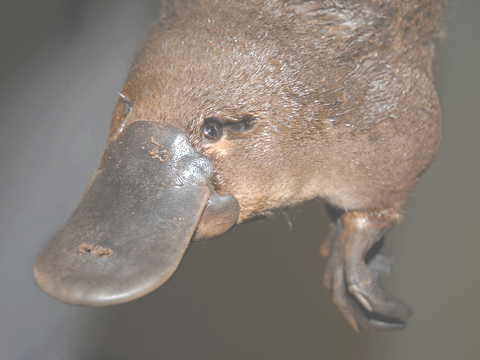
\includegraphics[width=3cm]{platypus}\\[-2ex]
      {\fontsize{3pt}{4pt}\selectfont http://www.sealifeconservation.org.au/adopt-an-animal/}
    \end{textblock*}

  \end{Beispiel}

  \onslide<+->

  \begin{block}{Ausweg}
    Verwende externe \enquote{Experten}
  \end{block}

\end{frame}

\begin{frame}

  \onslide<+->
  
  Exploration Übersicht
  
\end{frame}

\begin{frame}

  \onslide<+->
  
  Ende und Schluss
  
\end{frame}

\end{document}

%%% Local Variables: 
%%% mode: latex
%%% TeX-master: t
%%% ispell-local-dictionary: "de_DE"
%%% TeX-engine: xetex
%%% End: 

%  LocalWords:  Wikidata Concept Inclusions Konzeptnamen Rollennamen Konzeptinklusionen
%  LocalWords:  Ableitungsoperatoren Konzeptinklusion Inclusion label current node at of
%  LocalWords:  style opacity context induced base
